\documentclass[a4paper,11pt]{article}
\usepackage{fullpage}
\usepackage{graphicx}
\usepackage{eqnarray,amsmath, amssymb}
\usepackage{bookmark}
\usepackage{hyperref}

\usepackage{listings}
\usepackage{changepage}

\makeatletter
\renewcommand\@seccntformat[1]{}
\makeatother
\hypersetup{pdfinfo={
Title = {ELEN3007-Assignment-2024},
Author = {Kgadile "Naar-Kie" Masemola},
CreationDate = {D:202409120836},
%ModDate = {D:202409040530},
Subject = {ELEN3XXX Paper Format, 2024}
%/Keywords (ELEN3007, naar_kie, paper, project)
}}

%%%%%%%%%%%%%%%%%%%%%%%%%%%%%%%%%%%%%%%%%%%%%%%%%%%%%%%%%%%%%%%%%%%%%%%%%%%%%%%%%%%%%%%%%%%%

\title{ELEN3007A Group \underline{27} - Assignment 2024: \\ 
\large \emph{Application of Bayes’ Theorem for Locating a Robot’s
Position in an Enclosed Area}}
\author{Kgadile E Masemola (876729)}
\date{September 13, 2024}

\begin{document}
\maketitle

\section{QUESTION 1:}  Why does $\theta_k$ not lie between $- \pi$ and $\pi$ for which $p(\theta_k | \alpha, \beta, B)$ would then be $\frac{1}{2\pi}$?

\subsection{Solution 1:}
The given setup of the problem assumes that the photodetectors are placed on the x-axis above which the robot is located. Therefore, the signal comes from one side of the axis. This thus limits the range of the detectors to be within the range of $\pi$ (that is $-\frac{\pi}{2}$ to $\frac{\pi}{2}$). 

\section{QUESTION 2:}
Prove that
\begin{equation}
	p(x_k | \alpha, \beta, B) = \frac{\beta}{\pi (\beta^2 + (x_k - \alpha)^2)}
\end{equation}
\subsection{Solution 2:}
Using the relation $x_k = \alpha + \beta tan \theta_k$ (given in the brief) and the prior PDF $p(\theta_k | \alpha, \beta, B) = f_{\Theta | \Lambda, \beta, B}(\theta) = \frac{1}{\pi}$ and the transformation of random variables (notations for random variables defined \hyperref[sec:notation]{Solution 8})

\section{QUESTION 3:}
Plot $p(x_k | \alpha, \beta, B)$ and then relate its width at half maximum to the parameters of the PDF.

\subsection{Solution 3:}
The plot of the PDF $ p(x_k | \alpha, \beta, B) \Rightarrow f_{X | \Lambda, \beta, B}(x_k | \alpha, \beta = b)$ is shown in Figure 1 below. The \emph{parameters} are chosen to be $\alpha = 4; \beta = 2$ for $\{x_k \}^ {10} _{k = -10}$. It shows that the maximum value is when $x_k = 4 = \alpha$. At half maximum of \emph{these} paramaters, the width at half maximum of the distribution is $4 = 2 \beta$, half maximum height is $y = 0.1591536$.

\begin{figure}
        \centering
        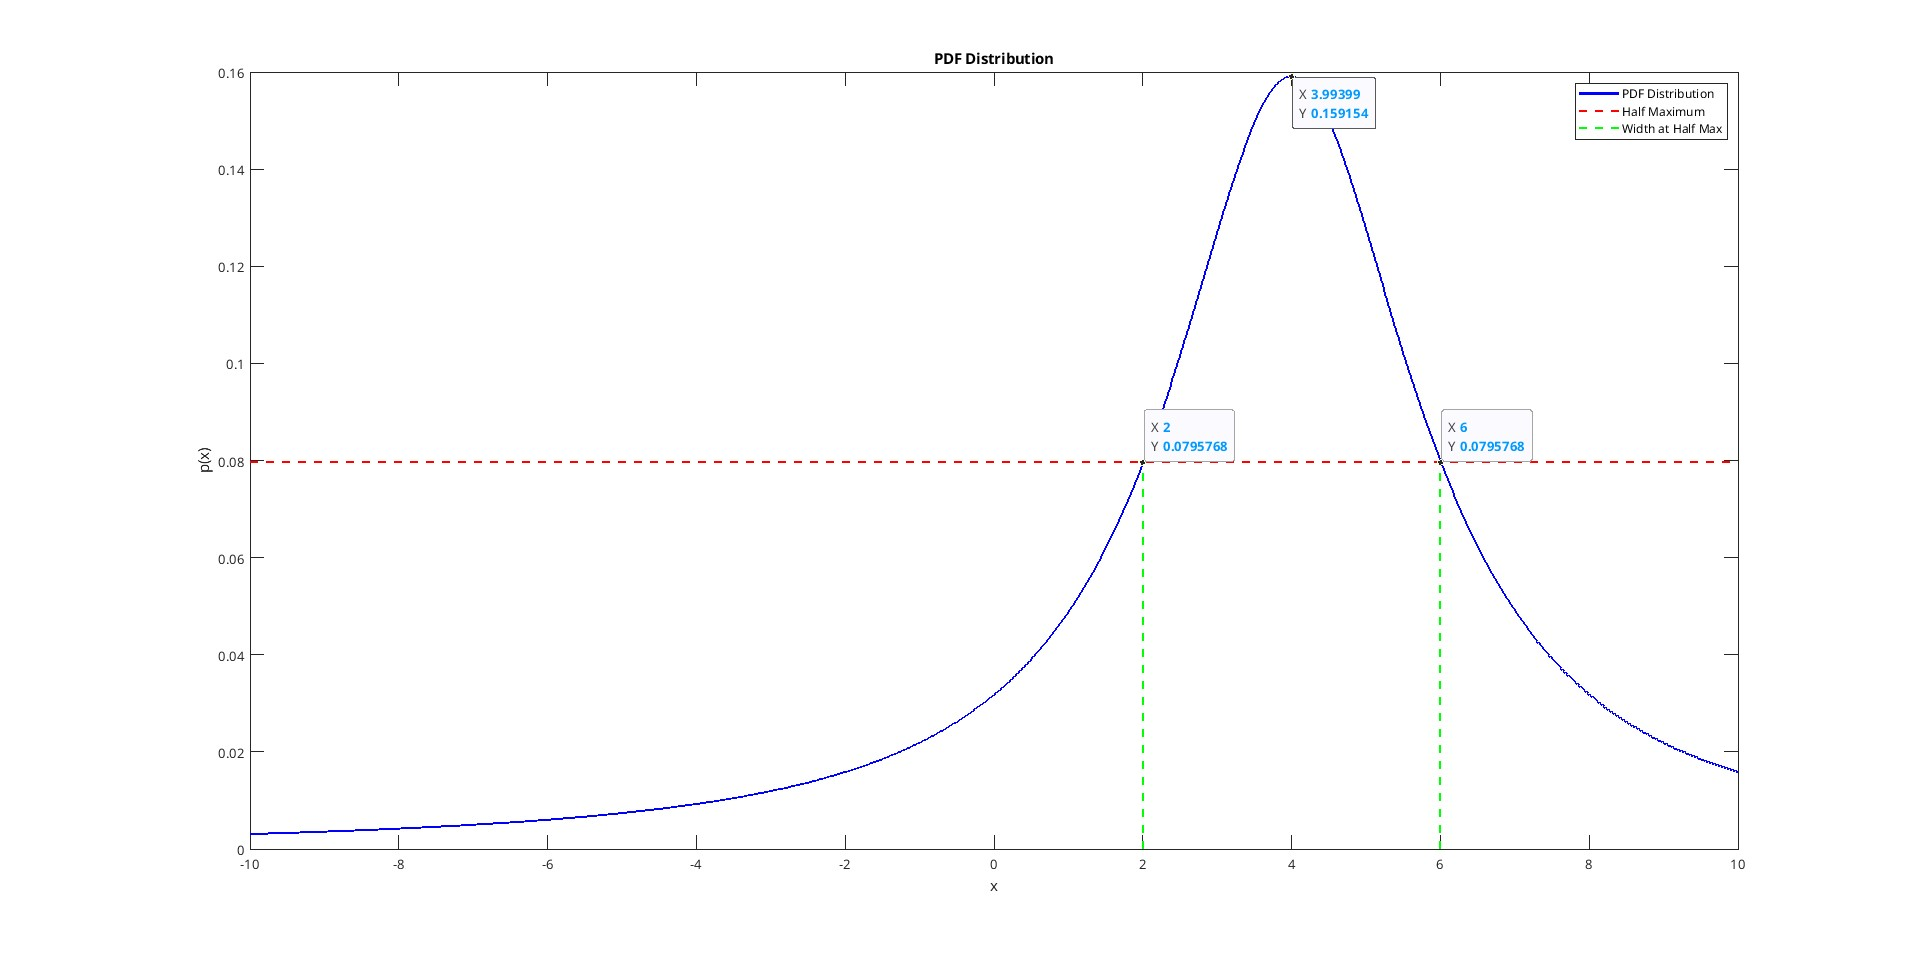
\includegraphics[scale=0.16]{q03pdfplot.jpg} 
        \caption{Plot of the PDF $p(x_k | \alpha, \beta, B)$}
\end{figure}


\section{QUESTION 4:}
Derive the expression for $p(\alpha | x_k, \beta, B)$.

\subsection{Solution 4:}
,

\section{QUESTION 5:}
Finally derive an expression for $p(\alpha | \{x_k\}^N _{k = 1}, \beta, B)$. (State all assumptions.)

\subsection{Solution 5:}
,

\section{QUESTION 6:}
Explain how one obtains the $x$-position of the robot from the result in (5.).

\subsection{Solution 6:}
,

\section{QUESTION 7:}
Implement the Bayesian position inference scheme in Matlab. Assume the robot is
located inside a confined square region of size $10$m $\times$ $10$m. Demonstrate your Bayes
estimator by inferring the robot’s $x$-position from the data/measurements $\{ x_k \}^{200} _{k = 1}$ in \emph{BayesData.mat}, with the robot’s $y$-position 4.5 m. Plot the Bayes posterior distribution for the first $N = 1, 2, 5$ and $30$ measurements. For this data, what is your best $x$-position estimate?

\subsection{Solution 7:}
,

\section{QUESTION 8:}
The notation presented above, deliberately does \emph{not} follow the conventions your Probs
lecturer introduced. Throughout your assignment, strictly use the notation prescribed for
use in Probs.
\subsection{Solution 8:}
\label{sec:notation}
Yes with the following Equations and Notations: 
 	\begin{eqnarray}
		p(\theta_k | \alpha, \beta, B) = f_{\Theta | \Omega, \beta, B}(\theta)\\
		p(x_k |\alpha, \beta, B) = f_{X | \Lambda, \mathfrak{B}, B}(\, \cdot \, | \alpha, \beta)\\
		\Lambda (\cdot) = \alpha;\: \mathfrak{B}(\cdot) = \beta ; \: X(\cdot) = x_k; \: \Theta ( \cdot) = \theta_k 
	\end{eqnarray}

\section{QUESTION 9:}
Professional report with clear and effective data representation. The report must not have
a title page and is not allowed to exceed 5 pages in length.
\subsection{Solution 9:}
The report is presented in homework assignment form(statement and solution). Additionally, the following reference materials have been consulted for the assignment: \cite{leon2017probability}, \cite{bishop2006pattern}

\section{(Bonus) QUESTION 10:}
Infer both the $x$-position as well as the $y$-position of the robot. Estimate both $\alpha$ and $\beta$ for the PDF in Eq. (1).
\subsection*{Solution 10:}



\bibliographystyle{unsrt}
\bibliography{elen3007ref}

\newpage
\appendix

\makeatother
\section{Appendix A. - Matlab Inference Scheme Code}
\begin{lstlisting}
% Load the data
load('BayesData.mat');
\end{lstlisting}

\newpage
\section{Appendix B. - Matlab Scheme Plots}
	Plots


\end{document}